%-*- coding:utf-8 -*-

\title{ALPSチュートリアル -- 概要}

\begin{document}

\lstset{language={C++},showspaces=false,rulecolor=\color[cmyk]{0, 0.29,0.84,0}}

\begin{frame}
  \titlepage
\end{frame}

\section*{Outline}
\begin{frame}[t,fragile]
  \tableofcontents
\end{frame}

\section{参考資料 / Reference Materials}
\subsection*{\redb\whiteb\greenb}

\begin{frame}[t,fragile]{ALPS参考資料}
  \begin{itemize}
    \setlength{\itemsep}{1em}
  \item ALPSチュートリアル資料
    \begin{itemize}
    \item CCMSハンズオン資料(日/英)
      
      [PDF]: {\footnotesize \url{http://sf.net/projects/alps-tutorial/files/}}
      
      [\TeX soruce]: {\footnotesize \url{https://github.com/cmsi/alps-tutorial/}}
      
     \item ALPSオフィシャルページTurorials (英/日): {\footnotesize \url{http://alps.comp-phys.org/}}
    \end{itemize}
  \item ALPS Developer Wiki (en): {\footnotesize \url{http://alps.comp-phys.org/trac/}}
  \item MateriApps (日/英): {\footnotesize \url{http://ma.cms-initiative.jp/listapps/alps}}
  \item 藤堂,「``実験技術''としての量子多体シミュレーションソフトウェアALPS」, \href{http://www.jps.or.jp/books/gakkaishi/2015/04/06/70-04exp.pdf}{日本物理学会誌 {\bf 70}, 275 (2015)}.
  \end{itemize}
\end{frame}

\begin{frame}[t,fragile]{ALPS論文}
  \begin{itemize}
    \setlength{\itemsep}{1em}
  \item F. Alet et al. {\it The ALPS Project: Open Source Software for
    Strongly Correlated Systems}, \href{http://jpsj.ipap.jp/link?JPSJS/74S/30}{J. Phys. Soc. Jpn. Suppl. 74, 30 (2005)}.
  \item A.~F. Albuquerque et al. {\it The ALPS project release 1.3: open source software for strongly correlated systems}, \href{http://dx.doi.org/10.1016/j.jmmm.2006.10.304}{J. Mag. Mag. Mat. 310, 1187 (2007)}.
  \item B. Bauer et al. {\it The ALPS project release 2.0: Open source software for strongly correlated systems}, \href{http://iopscience.iop.org/1742-5468/2011/05/P05001}{J. Stat. Mech., P05001 (2011)}.
  \item (A.~E. Antipov et al. {\it Updated Core Libraries of the ALPS Project}, \href{http://dx.doi.org/10.1016/j.cpc.2016.12.009}{Comp. Phys. Comm {\bf 213}, 235--251 (2017)}.)
  \end{itemize}
\end{frame}

\begin{frame}[t,fragile]{困った時は…}
  \begin{itemize}
    \setlength{\itemsep}{1em}
  \item 日本ALPSサポートチーム: {\href{mailto:alps@exa.phys.s.u-tokyo.ac.jp}{alps@exa.phys.s.u-tokyo.ac.jp}}
  \item MateriApps ALPS フォーラム(日/英):

    {\footnotesize \href{http://ma.cms-initiative.jp/ja/community/materiapps-messageboard/alps}{http://ma.cms-initiative.jp/ja/community/materiapps-...}}
  \item ALPS User's Mailing List (英):

    {\footnotesize \href{https://alps.comp-phys.org/mediawiki/index.php/Forum:Overview}{https://alps.comp-phys.org/mediawiki/index.php/Forum...}}
  \end{itemize}
\end{frame}

\begin{frame}[t,fragile]{ALPSチュートリアル スタッフ}
  \begin{itemize}
    \setlength{\itemsep}{1em}
  \item チュートリアル資料作成・講師
    \begin{itemize}
    \item 藤堂眞治 (東大院理/物性研)
    \item 本山裕一 (東大物性研)
    \end{itemize}
  \item 主催
    \begin{itemize}
    \item ISSP-CCMS: 東京大学物性研究所計算物質科学研究センター \url{http://ccms.issp.u-tokyo.ac.jp/} \\[2em]
    \end{itemize}
  \item これまでの協力者: 松尾春彦 (現 ペジーコンピューティング)、五十嵐亮 (現 東大情報基盤センター)、諏訪秀麿 (東大院理・テネシー大)、坂下達也 (現 名古屋大学)
  \end{itemize}
\end{frame}

\begin{frame}[t,fragile]
  \frametitle{チュートリアルの流れ}
             {\footnotesize\color{red} ◎}: 初心者コース (1〜2時間)

             {\footnotesize\color{blue} ◎}: 中級者コース (半日)

             {\footnotesize\color{green} ◎}: 開発者コース (半日〜全日) \\[1em]
             
  \begin{tabular}{|l|l|c|c|c|}
        \hline
        ALPSの概要 & {\tt 01\_overview} & {\footnotesize\color{red} ○} & {\footnotesize\color{blue} ◎} & {\footnotesize\color{green} ◎} \\
        \hline
        ALPSのインストール & {\tt 02\_installation} & {\footnotesize\color{red} } & {\footnotesize\color{blue} ○} & {\footnotesize\color{green} ◎} \\
        \hline
        アプリケーション実習(1) & {\tt 03\_tutorial} & {\footnotesize\color{red} ◎} & {\footnotesize\color{blue} ◎} & {\footnotesize\color{green} ○} \\
        \hline
        Python入門 & {\tt 04\_python} & {\footnotesize\color{red}} & {\footnotesize\color{blue} ○} & {\footnotesize\color{green} ○} \\
        \hline
        ALPS Python入門 & {\tt 05\_pyalps} & {\footnotesize\color{red} } & {\footnotesize\color{blue} ○} & {\footnotesize\color{green} ○} \\
        \hline
        Matplotlib入門 & {\tt 06\_matplotlib} & {\footnotesize\color{red} } & {\footnotesize\color{blue} ○} & {\footnotesize\color{green} ○} \\
        \hline
        アプリケーション実習(2) & & {\footnotesize\color{red} } & {\footnotesize\color{blue} ◎} & {\footnotesize\color{green} } \\
        \hline
        アプリケーションのALPS化 & {\tt 07\_alpsize} & {\footnotesize\color{red} } & {\footnotesize\color{blue} } & {\footnotesize\color{green} ◎} \\
        \hline
  \end{tabular}
\end{frame}

\begin{frame}[t,fragile]
  \frametitle{ALPSチュートリアルの目標}
  \begin{itemize}
    \setlength{\itemsep}{1em}
    \item ALPSの概要を知る \ [{\footnotesize\color{red} ○}{\footnotesize\color{blue} ◎}{\footnotesize\color{green} ◎}]
    \item ALPSアプリケーションの実行方法を学ぶ  \ [{\footnotesize\color{red} ◎}{\footnotesize\color{blue} ◎}{\footnotesize\color{green} ○}]
    \item ALPS Pythonツールを使った結果の解析方法を学ぶ  \ [{\footnotesize\color{red} ○}{\footnotesize\color{blue} ○}{\footnotesize\color{green} ○}]
    \item ALPSライブラリの仕組みを学ぶ \ [{\footnotesize\color{red} ー}{\footnotesize\color{blue} ー}{\footnotesize\color{green} ○}]
    \item ユーザアプリケーションの作成方法を学ぶ \ [{\footnotesize\color{red} ー}{\footnotesize\color{blue} ー}{\footnotesize\color{green} ◎}]
    \item (ALPSチュートリアルの問題点を洗い出し改良する) \ [{\footnotesize\color{red} ◎}{\footnotesize\color{blue} ◎}{\footnotesize\color{green} ◎}] 
  \end{itemize}
\end{frame}

\section{量子格子模型 / Quantum Lattice Models}
\subsection*{\redb\whiteb\greenb}

\begin{frame}[fragile]{量子格子模型}
  \begin{columns}[T]
    \begin{column}{.8\textwidth}
      \begin{itemize}
        \setlength{\itemsep}{-.5em}
      \item 量子スピン模型(XXZ模型) \begin{equation*} {\cal H} = \frac{J^{xy}}{2}
        \sum_{\langle i,j \rangle} (S^+_i S^-_j + S^-_i S^+_j) + J^z
        \sum_{\langle i,j \rangle} S^z_i S^z_j \end{equation*}
      \item Hubbard模型 (fermionic / bosonic)
        \begin{equation*} {\cal H} = -t \sum_{\langle i,j \rangle \sigma}
        (c^\dagger_{i\sigma} c_{j\sigma} + \mbox{h.c.}) + U \sum_{i}
        n_{i\uparrow} n_{i\downarrow} \end{equation*}
      \item t-J模型 \begin{equation*} {\cal H} = -t \sum_{\langle i,j \rangle \sigma}
        (c^\dagger_{i\sigma} c_{j\sigma} + \mbox{h.c.}) + J \sum_{i,j}
        ({\bf S}_i \cdot {\bf S}_j - n_{i} n_{j} / 4) \end{equation*}
      \end{itemize}
    \end{column}
    \begin{column}{.2\textwidth}
      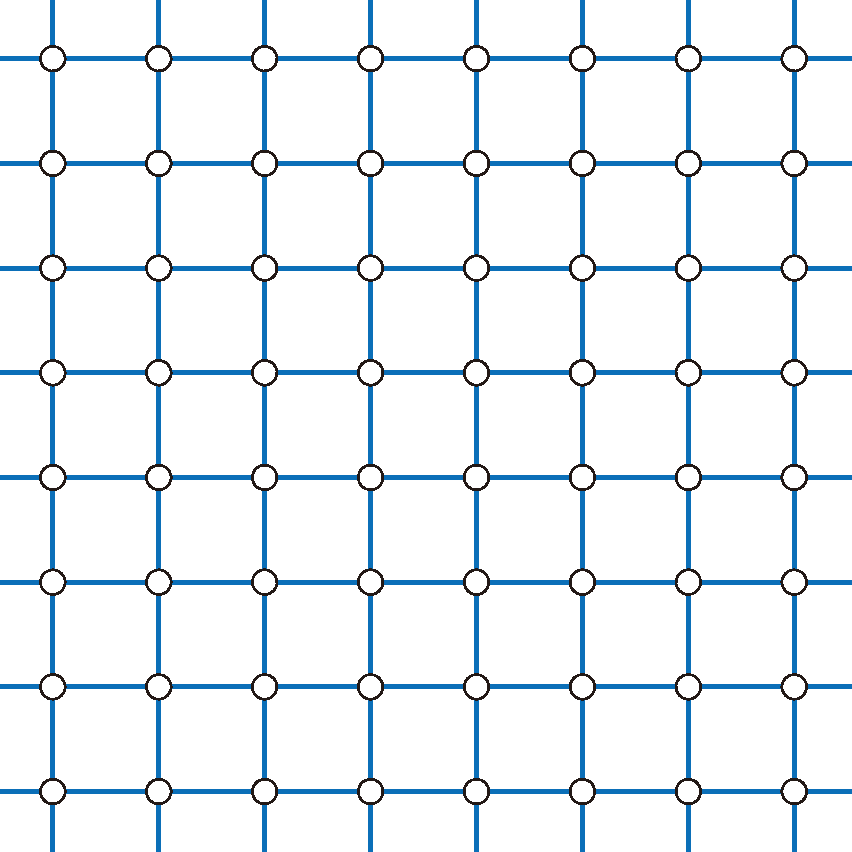
\includegraphics[width=\textwidth]{square.pdf}
    \end{column}
  \end{columns}
\end{frame}

\begin{frame}[t,fragile]{なぜ量子格子模型を考えるのか?}
  \begin{columns}[T]
    \begin{column}{.2\textwidth}
      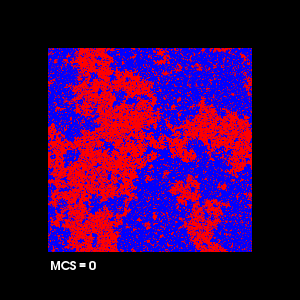
\includegraphics[width=\textwidth]{ising-tc.png} \\
      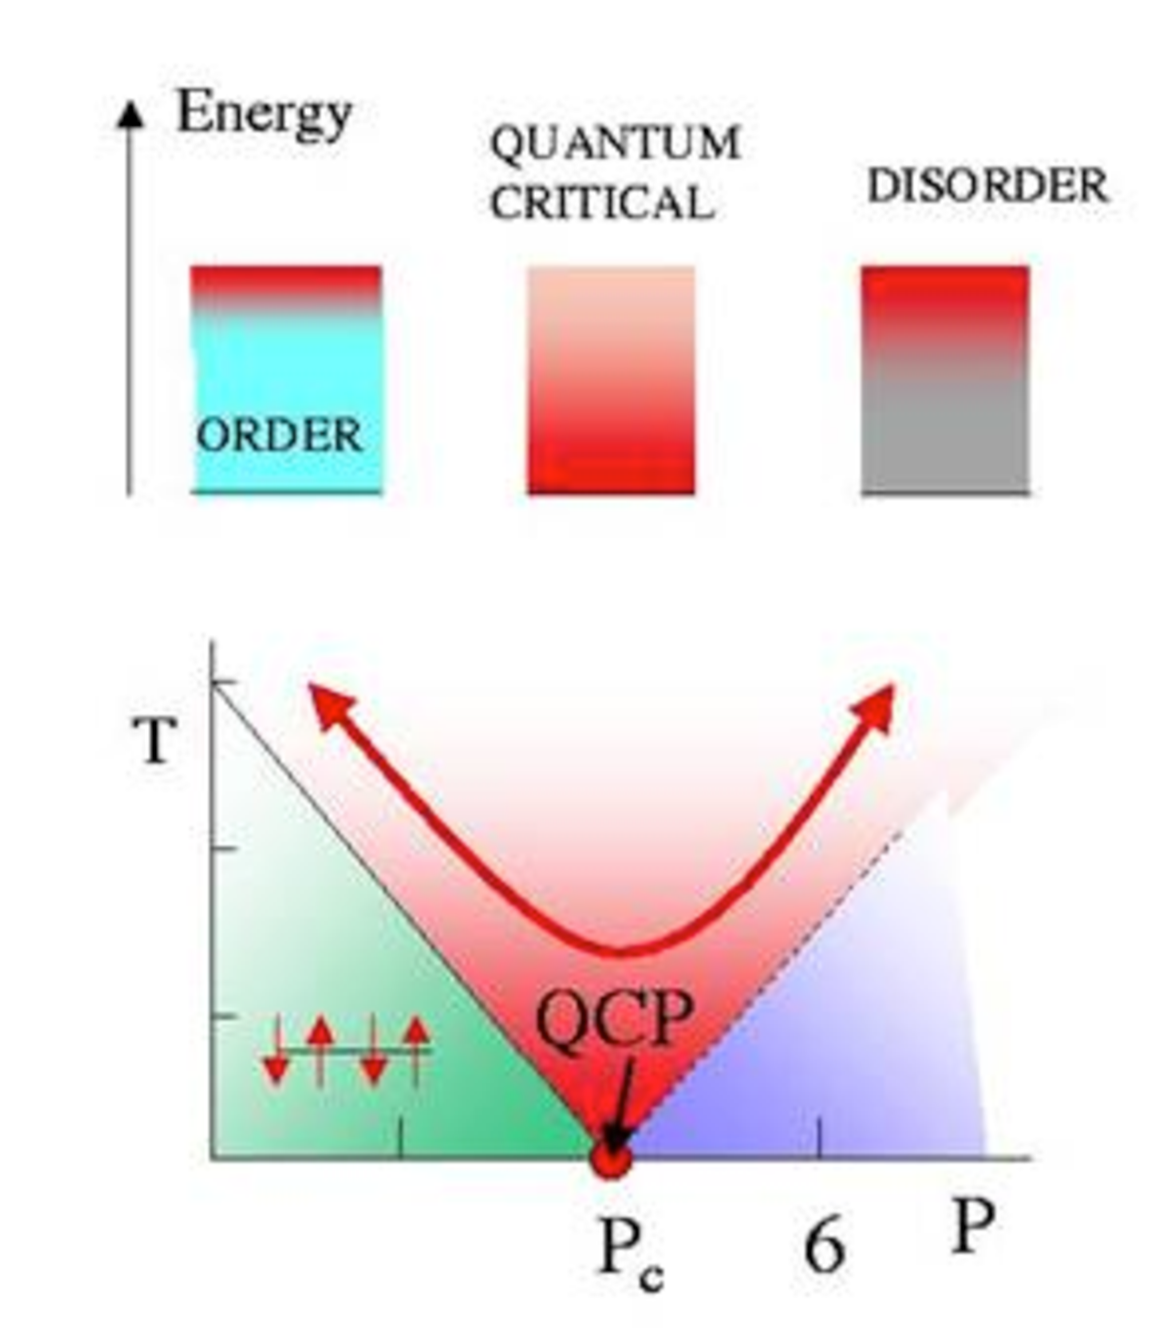
\includegraphics[width=\textwidth]{qcp.pdf}
    \end{column}
    \begin{column}{.8\textwidth}
      \begin{itemize}
        %\setlength{\itemsep}{1em}
      \item 量子多体系における強相関効果
        \begin{itemize}
        \item さまざまな秩序状態
        \item 量子的に強くゆらいだ相: 量子液体, スピンギャップ相
        \item 量子相転移, 量子臨界現象
        \end{itemize}
      \item 量子統計物理におけるユニバーサリティー
        \begin{itemize}
        \item 量子臨界現象は系の次元, 秩序変数の対称性などにしか依存しない
        \item 量子臨界現象特有のユニバーサリティークラスの探索
        \end{itemize}
      \item 新しい計算物理学的手法の発展
        \begin{itemize}
        \item 量子モンテカルロ法, DMRG, DMFT, テンソルネットワーク, など
        \end{itemize}
      \end{itemize}
    \end{column}
  \end{columns}
\end{frame}

\section{ALPSプロジェクト / ALPS Project}
\subsection*{\redb\whiteb\greenb}

\begin{frame}[t,fragile]{ALPSとは?}
  ALPS = \alert{A}lgorithms and \alert{L}ibraries for \alert{P}hysics \alert{S}imulations
  \begin{itemize}
  \item 量子スピン系, 電子系など強相関量子格子模型のシミュレーションのためのオープンソースソフトウェアの開発を目指す国際共同プロジェクト
    \begin{itemize}
    \item ALPSライブラリ = C++による格子模型のための汎用ライブラリ群
    \item ALPSアプリケーション = 最新のアルゴリズムに基づくアプリケーション群: QMC, DMRG, ED, DMFT等
    \item ALPSフレームワーク = 汎用入出力形式, 解析ツール, スケジューラなど, 大規模並列シミュレーションのための環境
    \end{itemize}
  \item 2002年開発開始
  \item 開発者: 20+名 (7+ヶ国)
  \item ソースコード: C++, Python, Fortran (400,000+行)
  \end{itemize}
\end{frame}

\begin{frame}[fragile]{はしご格子スピン系のモデリング: Na$_2$Fe$_2$(C$_2$O$_4$)$_3$(H$_2$O)$_2$}
  \begin{center}
    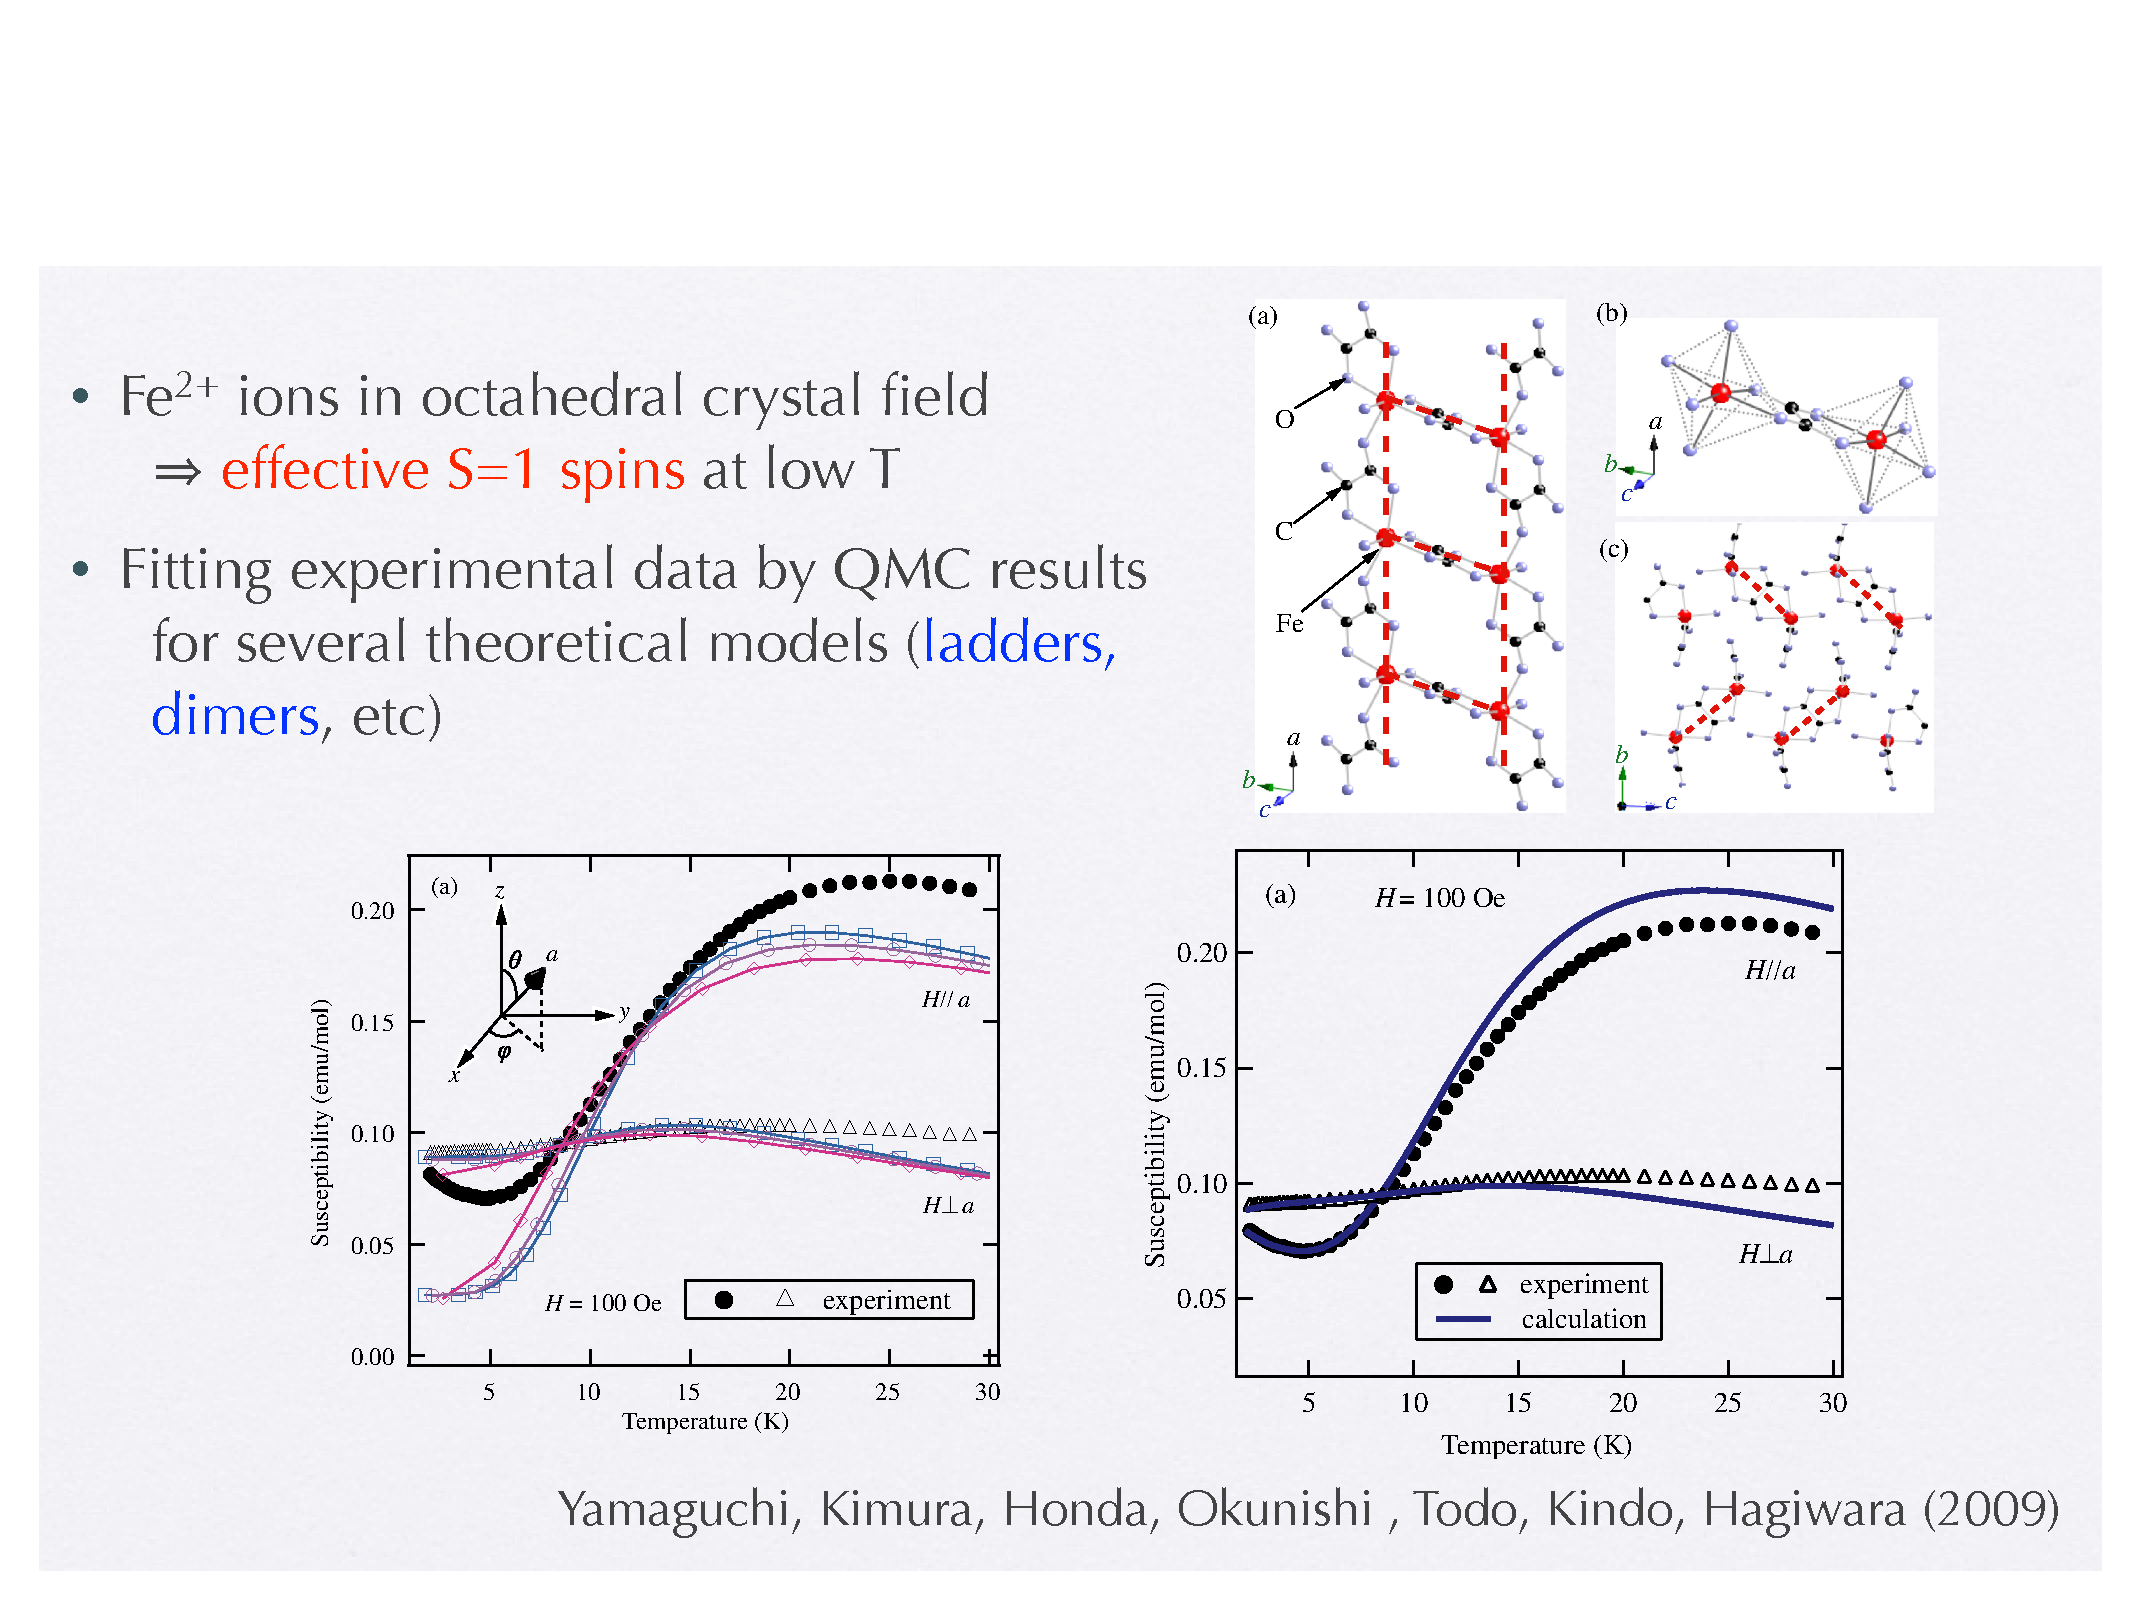
\includegraphics[height=.8\textheight]{ladder.pdf}
  \end{center}
\end{frame}

\begin{frame}[fragile]{拡張ボーズ・ハバード模型における超固体相}
  \begin{center}
    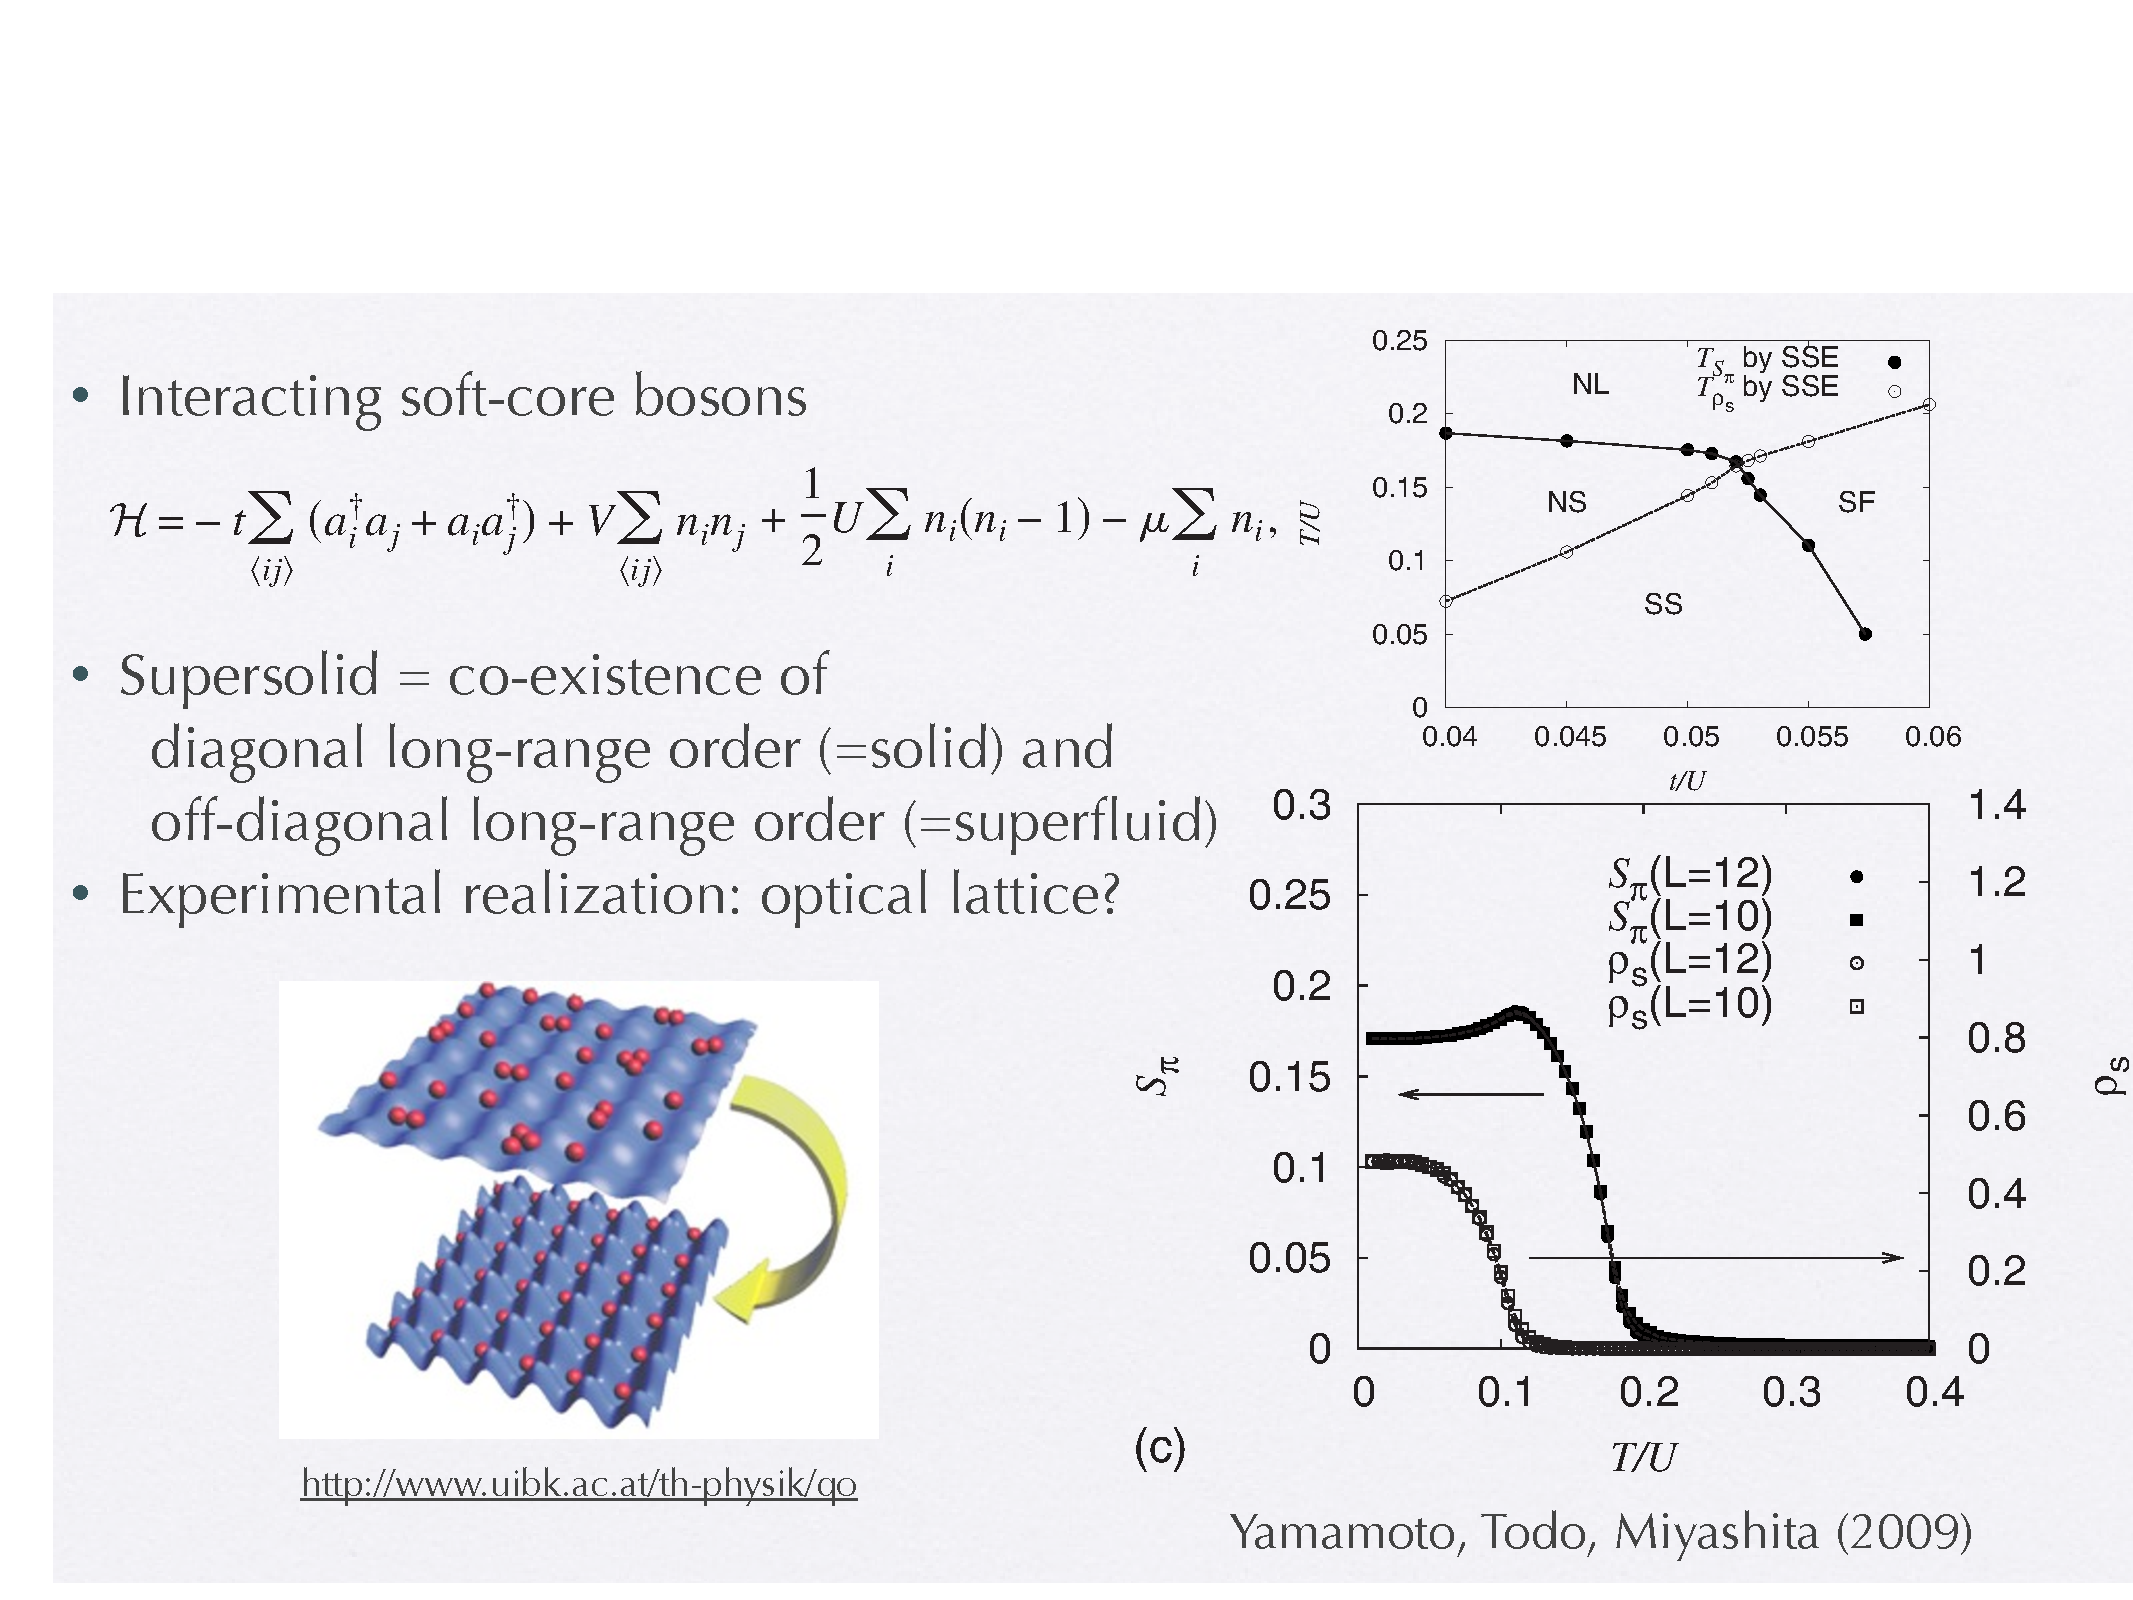
\includegraphics[height=.8\textheight]{supersolid.pdf}
  \end{center}
\end{frame}

\begin{frame}[t,fragile]{ターゲット・オーディエンス}
  \begin{itemize}
    \setlength{\itemsep}{1em}
  \item 実験家
    \begin{itemize}
    \item 物質のモデリングにソフトウェアパッケージを利用
    \item 実験結果とシミュレーション結果のフィッティングにより, 相互作用定数などを決定
    \end{itemize}
  \item 理論家
    \begin{itemize}
    \item 理論的なアイデアのチェックに使いやすい整備されたコードを利用
    \item 自前のコードのデバッグに
    \item 新しいコード開発の基盤としての利用
    \end{itemize}
  \item 計算機科学者, 学生, $\cdots$
  \end{itemize}
\end{frame}

\begin{frame}[t,fragile]
\frametitle{``Cite-me''ライセンス}
  \begin{itemize}
  \item GNU General Public License 2 (GPL2) を基本としたライセンス
  \item Non-commercial academic use の場合自由に利用可能
  \item 自由に再配布可
  \item ユーザが変更を施したコードも同じライセンスの下で再配布可
  \item ALPSを用いた研究成果を公表する場合には, acknowledgement と論文の引用をお願いします
    \begin{minipage}{.9\textwidth}
    \begin{block}{ALPSライブラリ/アプリケーションライセンスより抜粋}
      In any scientific publication based wholly or in part on the
      Library, the use of the Library must be acknowledged and the
      publications listed in the accompanying CITATIONS.txt document
      must be cited.
    \end{block}
    \end{minipage}
  \end{itemize}
\end{frame}

\begin{frame}[t,fragile]
  \frametitle{ALPSの特徴}
  \begin{itemize}
  \item {\color{red} 任意の}格子
    \begin{itemize}
    \item XMLフォーマットによる格子構造の定義
    \item ユニットセルの繰り返しによる格子生成
    \item 格子を任意の有限グラフ(頂点と辺の集合)として定義することも可能
    \end{itemize}
  \item {\color{red} 任意の}ハミルトニアン(模型)
    \begin{itemize}
    \item XMLフォーマットによる量子数、演算子の定義
    \item 数式によるハミルトニアンの定義
    \end{itemize}
  \item 様々な{\color{red} 最新の}解法(アプリケーション): ED, CMC, QMC, DMRG, DMFT
  \item {\color{red} 全ての}ALPSアプリケーションに共通の入力形式
  \item {\color{red} 汎用的な}出力形式、Pythonによる解析・グラフ作成ツール
  \end{itemize}
\end{frame}

\section{ALPSライブラリ / ALPS Libraries}
\subsection*{\redm\whiteb\greenb}

\begin{frame}[t,fragile]{ALPSの階層構造}
  \begin{center}
    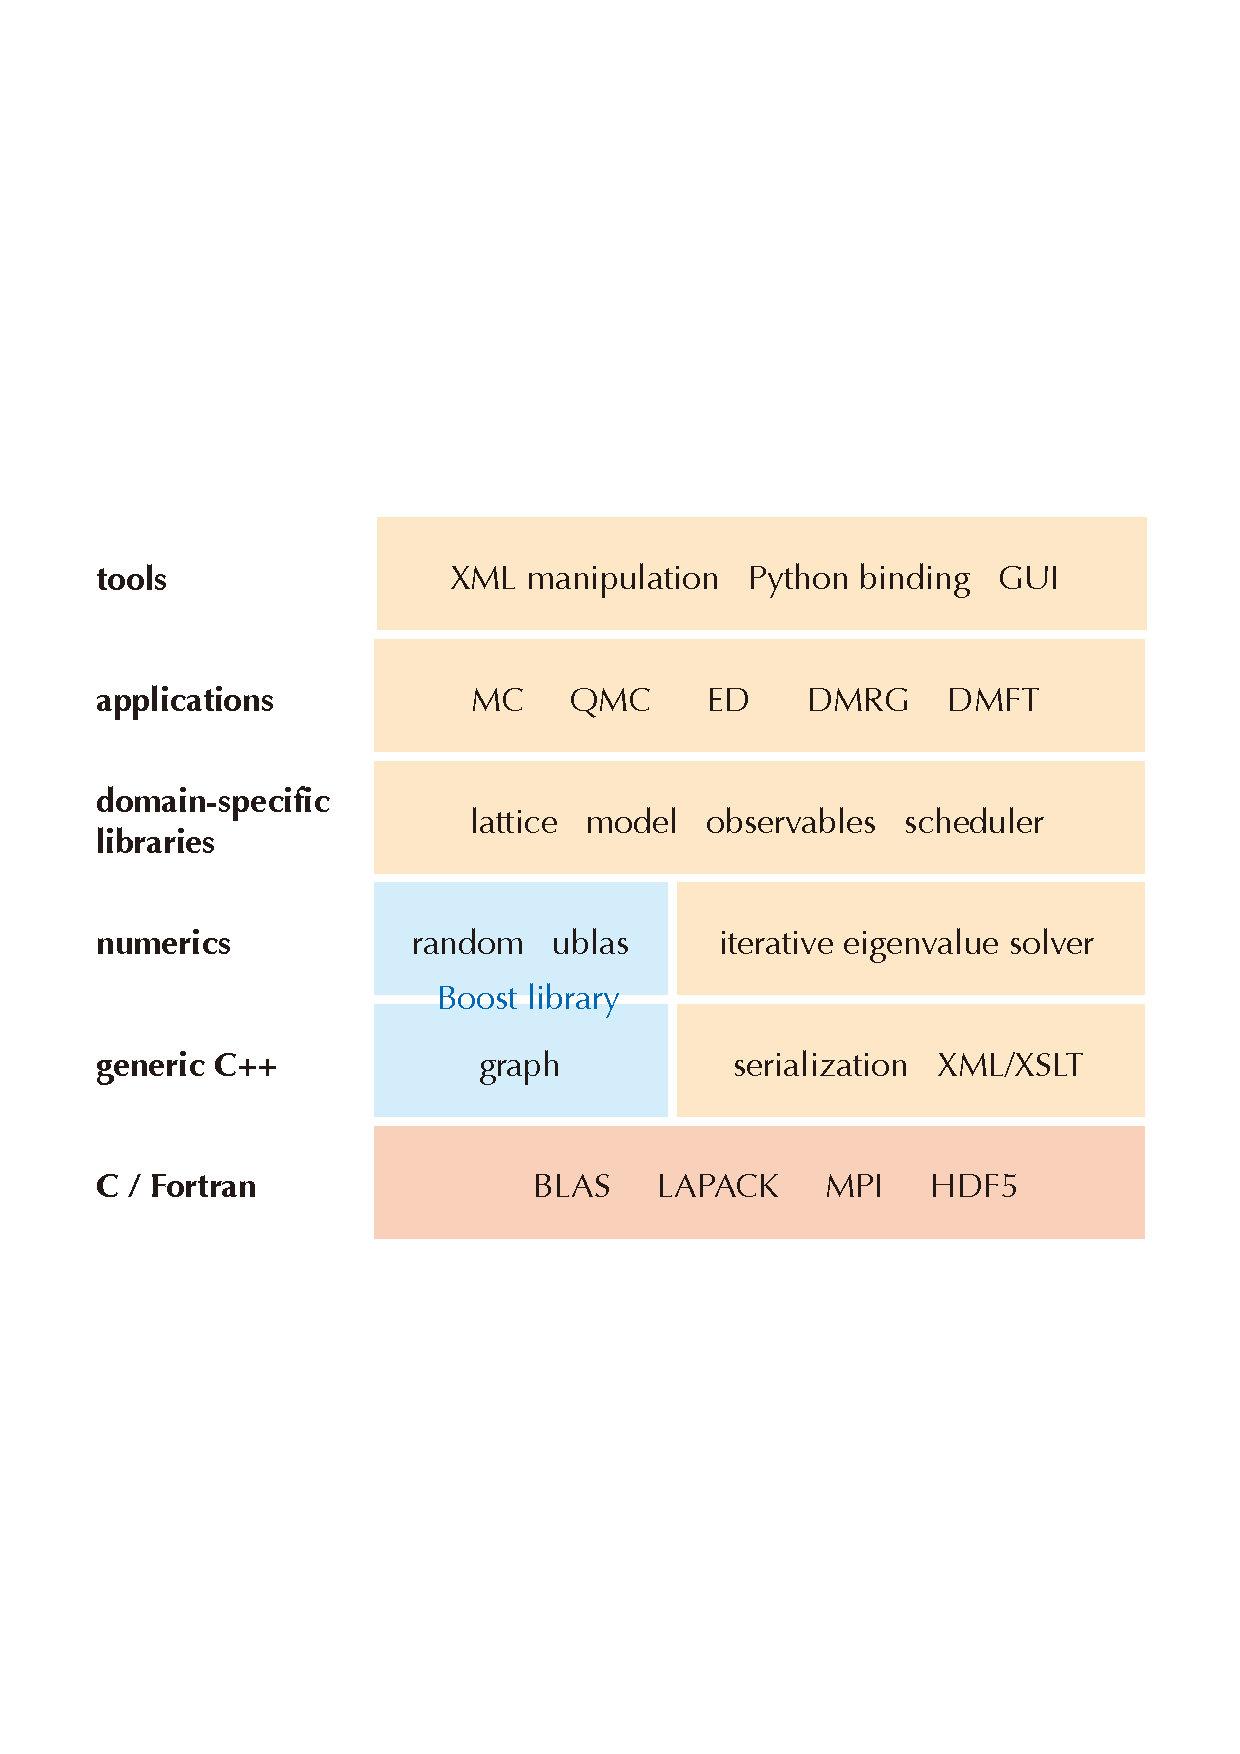
\includegraphics[height=0.65\textheight]{hierarchy.pdf}
  \end{center}
\end{frame}

\begin{frame}[t,fragile]
  \frametitle{サードパーティーのライブラリ}
  \begin{itemize}
    \setlength{\itemsep}{1em}
  \item \href{http://www.boost.org/}{Boost C++ Library}: 乱数, グラフ, シリアル化, など多くの有用なライブラリ群
  \item \href{http://www.hdfgroup.org/HDF5/}{HDF5} (Hierarchical Data Format): プラットフォーム非依存のバイナリファイル格納形式
  \item \href{http://www.mpi-forum.org/}{MPI} (Message Passing Interface): 並列計算のためのメッセージ通信 (オプション)
  \item \href{http://www.netlib.org/blas/}{BLAS}, \href{http://www.netlib.org/lapack/}{LAPACK}: 線形演算(行列対角化, 特異値分解など) (オプション)
  \end{itemize}
\end{frame}

\subsection*{\redb\whitem\greenb}

\begin{frame}[t,fragile]
  \frametitle{ALPS/parameterライブラリ}
  \begin{columns}[T]
    \begin{column}{.5\textwidth}
      \begin{itemize}
      \item パラメータの入出力のためのライブラリ
        %\begin{itemize}
        \item 改行, セミコロン, コンマで変数を区別
        \item 四則演算, 初等関数(sin, cos, expなど)が使える
        \item $\pi$ (PI), 虚数単位(I)
          \item C 風, C++風のコメント
          \item \{ \} で囲まない変数は共通パラメータ
          \item \{ \} で囲んだ変数は異なるパラメータセット
        %\end{itemize}
      \end{itemize}
    \end{column}
    \begin{column}{.5\textwidth}
    \begin{lstlisting}
LATTICE = "chain lattice";
L = 16,
SEED = 2873
// C++ style comment
SWEEPS = 4096;
THERMALIZATION = SWEEPS/8;
/* C style comment */
{ T = 2; Sq = 2*PI/3; }
{ T = 1.8; }
\end{lstlisting}
    \end{column}
  \end{columns}
\end{frame}

\begin{frame}[t,fragile]
  \frametitle{ALPS/parameterを使ったコード例}
  \lstset{language={C++}}
  \begin{lstlisting}
#include <boost/foreach.hpp>
#include <alps/parameter.h>
int main() {
  std::ifstream fin;
  fin.open("parameters.txt");
  alps::ParameterList plist(fin);
  BOOST_FOREACH(alps::Parameters& p, plist) {
    double a = p["a"];
    double b = p.value_or_default("b", 0.5);
    ...
  }
  ...
}
\end{lstlisting}
\end{frame}

\begin{frame}[t,fragile]
  \frametitle{ALPS/aleaライブラリ}
  \begin{itemize}
  \item マルコフ連鎖における平均値, 分散, 自己相関を計算するライブラリ
    \lstset{language={C++}}
    \begin{lstlisting}
alps::RealObservable mag2("Magnetization^2");
...
mag2 << m * m; // at each MC step
\end{lstlisting}
  \item ビンニング解析を用いた平均値, エラー, 自己相関時間の評価
    \lstset{language={C++}}
    \begin{lstlisting}
std::cout << mag2 << std::endl;
\end{lstlisting}
  \item 出力
\lstset{language={bash}}
\begin{lstlisting}
Magnetization^2: 3.142 +/- 0.001; tau = 10.3
\end{lstlisting}
  \end{itemize}
\end{frame}

\begin{frame}[t,fragile]
  \frametitle{ALPS/aleaライブラリ}
  \begin{itemize}
  \item ジャックナイフ法を用いた非線形量のエラー評価
    \lstset{language={C++}}
    \begin{lstlisting}
alps::RealObsevaluator mag2eval(mag2);
alps::RealObsevaluator mag4eval(mag4);
alps::RealObsevaluator binder = mag2eval * mag2eval / mag4eval;
std::cout << binder;
\end{lstlisting}
  \item 出力
\lstset{language={bash}}
\begin{lstlisting}
(Magnetization^2) * (Magnetization^2) / (Magnetization^4): 0.453 +/- 0.005
\end{lstlisting}
  \end{itemize}
\end{frame}

\subsection*{\redb\whiteb\greenb}

\begin{frame}[t,fragile,shrink]
  \frametitle{ALPS/latticeライブラリ}
  \begin{itemize}
    \setlength{\itemsep}{1em}
  \item 「格子構造」は数学的には「グラフ」で表現できる
    \begin{itemize}
    \item site $\Leftrightarrow$ vertex
    \item bond $\Leftrightarrow$ edge
    \end{itemize}
  \item Boost Graph Library に対する「ラッパー」を提供
    \begin{itemize}
    \item XMLによる「格子構造」の入出力
    \item 「ユニットセル」による繰り返し構造の指定
    \item 座標, パリティ, 逆格子ベクトルなどの属性
    \end{itemize}
  \item あらかじめ用意されている格子: ``hain lattice", ``square lattice", ``triangular lattice", ``honeycomb lattice", ``simple cubic lattice", など
  % \item ``printgraph'' で格子のチェック
  \end{itemize}
\end{frame}

\begin{frame}[t,fragile]
  \frametitle{有限格子 + ユニットセルの埋め込み}
  \begin{itemize}
  \item 格子の指定
  \begin{lstlisting}
<LATTICE name="2D" dimension="2">
  <BASIS>
    <VECTOR>   1 0 </VECTOR>
    <VECTOR> 0.5 1 </VECTOR>
  </BASIS>
</LATTICE>
\end{lstlisting}
  \end{itemize}
  \begin{center}
    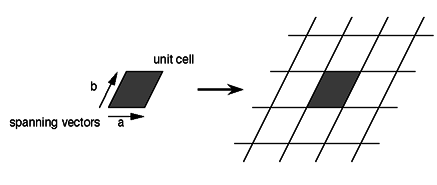
\includegraphics[height=0.3\textheight]{TutorialLatticeHOWTOLattice1}
  \end{center}
\end{frame}

\begin{frame}[t, fragile]
  \frametitle{有限格子 + ユニットセルの埋め込み}
  \begin{itemize}
  \item ユニットセル
  \begin{lstlisting}
<UNITCELL name="simple1d" dimension="1" vertices="1">
  <EDGE>
    <SOURCE vertex="1" offset="0"/><TARGET vertex="1" offset="1"/>
  </EDGE>
</UNITCELL>
\end{lstlisting}
  \end{itemize}
  \begin{center}
    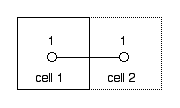
\includegraphics[height=0.25\textheight]{TutorialLatticeHOWTOLatticegraph3}
  \end{center}
\end{frame}

\begin{frame}[t,fragile]
  \frametitle{有限格子 + ユニットセルの埋め込み}
  \begin{itemize}
  \item サイズ, 境界条件の指定
    \begin{lstlisting}
<LATTICEGRAPH name = "chain lattice">
  <FINITELATTICE>
    <LATTICE ref="chain lattice"/>
    <PARAMETER name="L"/>
    <EXTENT size ="L"/>
    <BOUNDARY type="periodic"/>
  </FINITELATTICE>
  <UNITCELL ref="simple1d"/>
</LATTICEGRAPH>
\end{lstlisting}
  \item より複雑な格子の作り方
    \begin{itemize}
    \item ALPS Lattice HOWTO: {\small \href{http://alps.comp-phys.org/mediawiki/index.php/Tutorials:LatticeHOWTO/ja}{http://alps.comp-phys.org/mediawiki/ index.php/Tutorials:LatticeHOWTO/ja}}
    \end{itemize}
  \end{itemize}
\end{frame}

\begin{frame}[t,fragile]
  \frametitle{ALPS/modelライブラリ}
  \begin{itemize}
%    \setlength{\itemsep}{1em}
  \item XMLを使ってハミルトニアンを定義する
    \begin{itemize}  
    \item 量子数や演算子の定義
    \item シンボリックな表現を使って, ハミルトニアンのサイト項やボンド項を定義
    \end{itemize}
    \begin{lstlisting}
Jz*Sz(i)*Sz(j)+Jxy/2*(Splus(i)*Sminus(j)+Sminus(i)*Splus(j))
\end{lstlisting}
  \item 作成した局所ハミルトニアンは行列の形で取り出せる
  \item プラケット項などの多サイトにわたる相互作用には未対応
  \item ALPS Model HOWTO: {\small \href{http://alps.comp-phys.org/mediawiki/index.php/Tutorials:ModelHOWTO/ja}{http://alps.comp-phys.org/mediawiki/ index.php/Tutorials:ModelHOWTO/ja}}
  \item あらかじめ用意されている模型: ``spin", ``boson Hubbard", ``hardcore boson", ``fermion Hubbard", ``alternative fermion Hubbard", ``spinless fermions", ``Kondo lattice", ``t-J"
  \end{itemize}
\end{frame}

% \section{ALPS/scheduler}

% \section{HDF5とは?}

\section{ALPSアプリケーション / ALPS Applications}
\subsection*{\redb\whiteb\greenb}

\begin{frame}[t,fragile]
  \frametitle{ALPSアプリケーション}
  \begin{description}
  \item[fulldiag] 厳密対角化(全対角化法)
  \item[sparsediag] 厳密対角化(Lanczos法)
  \item[spinmc] 古典モンテカルロ法
  \item[simplemc] 古典モンテカルロ法
  \item[loop] 量子モンテカルロ法(ループアルゴリズム)
  \item[dirloop\_sse] 量子モンテカルロ(向き付きループアルゴリズム)
  \item[worm] 量子モンテカルロ(ワームアルゴリズム)
  \item[dmrg,tebd] 密度行列繰り込み群
  \item[hirshfye,interaction,hybridization] 動的平均場近似のQMCソルバ
  \end{description}
\end{frame}

\begin{frame}[t,fragile]
  \frametitle{厳密対角化・古典モンテカルロ法}
  \begin{description}
  \item[fulldiag] 厳密対角化(全対角化法)
    \begin{itemize}
    \item ハウスホルダー法を用いて量子格子模型の全てのエネルギー固有値・固有状態と任意の温度における物理量を計算
    \end{itemize}
  \item[sparsediag] 厳密対角化(Lanczos法)
    \begin{itemize}
    \item ランチョス法を用いて, 基底状態と少数の低励起状態を求める
    \end{itemize}
  \item[spinmc] 古典モンテカルロ法
    \begin{itemize}
      \item メトロポリス法あるいはクラスターアルゴリズム
      \item 古典スピン模型のモンテカルロシミュレーション
      \item 磁場中のイジング模型, XY模型, ハイゼンベルグ模型, ポッツ模型
    \end{itemize}
  \item[simplemc] 古典モンテカルロ法によるイジング模型, XY模型, ハイゼンベルグ模型の計算
  \end{description}
\end{frame}

\begin{frame}
  \frametitle{量子モンテカルロ法}
  \begin{description}
  \item[loop] ループアルゴリズム量子モンテカルロ
    \begin{itemize}
      \item 連続虚時間ループアルゴリズム
      \item 時間反転対称性を持つ系(零磁場の場合、横磁場イジング模型など)に有効
      \item 2点相関関数(グリーン関数を含む)の計算
    \end{itemize}
  \item[dirloop\_sse] 向き付きループアルゴリズム量子モンテカルロ
    \begin{itemize}
      \item SSE (Stochastic Series Expansion)表示
      \item 磁場中スピン模型, ボーズハバード模型などに有効
    \end{itemize}
  \item[worm] ワームアルゴリズム量子モンテカルロ
    \begin{itemize}
      \item 連続虚時間表示ワームアルゴリズム
      \item 非常に強い磁場が存在する場合などに有効
    \end{itemize}
  \end{description}
\end{frame}

\begin{frame}
  \frametitle{密度行列繰り込み群・動的平均場}
  \begin{description}
  \item[dmrg,tebd] 密度行列繰り込み群
    \begin{itemize}
      \item 一次元系・擬一次元系の基底状態および低励起状態を計算
      \item 局所的な物理量や2点相関関数の測定
      \item エンタングルメントエントロピーの測定
    \end{itemize}
  \item[hirshfye,interaction,hybridization] 動的平均場近似のQMCソルバ
    \begin{itemize}
      \item 系の自己エネルギーの波数依存性を無視することで, 多体フェルミオン模型を不純物問題に帰着
      \item Hirsch-Fye法 ({\tt hirshfye})
      \item 相互作用展開 ({\tt interaction})
      \item 混成状態展開 ({\tt hybridization})
    \end{itemize}
  \end{description}
\end{frame}

\end{document}
